\documentclass[11pt]{article}

\usepackage[utf8]{inputenc}  
\usepackage{amsmath}         
\usepackage{amssymb}         
\usepackage{graphicx}        
\usepackage{geometry}        
\usepackage{fancyhdr}        
\usepackage{hyperref}       
\usepackage{float} 
\usepackage{xcolor}
\usepackage{ulem}
\usepackage{tabularx}
\usepackage{cancel}
\usepackage{multicol}


% Impostazioni per i margini
\geometry{a4paper, margin=0.8in}

% Intestazioni
\pagestyle{fancy}
\fancyhf{}
\fancyhead[L]{Linguaggi Formali e Compilatori}
\fancyhead[R]{Soluzione Esercizi Tipo - Parte III}
\fancyfoot[C]{\thepage}   
\setlength{\headheight}{14pt}


\begin{document}
\section{Esercizio 1}
\subsection*{Soluzione}
Gli items di $J[Aa]$ sono: 
$$S \rightarrow Aa\cdot B$$
$$B \rightarrow \cdot$$
Per lo svolgimento guardare la soluzione al primo esercizio degli "Esercizi Tipo - Parte II".
Riporto l'automa.

\hypertarget{automa_1}{}
\begin{figure}[H]
\centering
  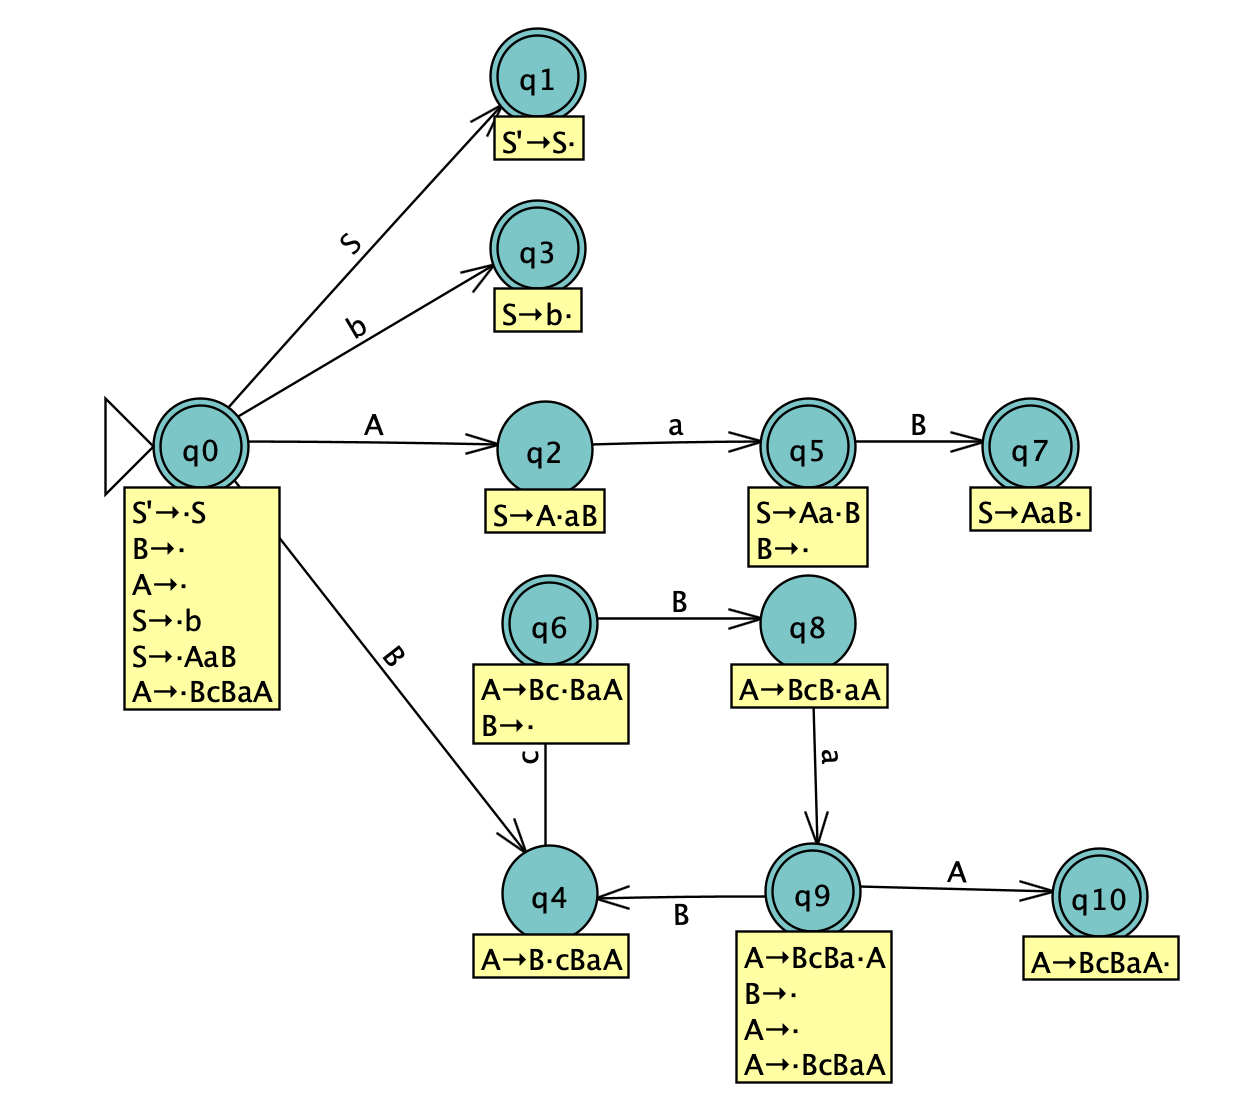
\includegraphics[width=0.6\textwidth]{../2/img/01AutomaSRL.png}
  \label{fig:01-automa}
\end{figure}
\section{Esercizio 2}
\subsection{Soluzione}
Seguendo le transazioni dallo stato iniziale dell'automa \hyperlink{automa_1}{$\cal A$} 
si arriva allo stato 6 dell'automa, che non presenta alcun conflitto.
Rimando sempre al primo esercizio delgli "Esercizi Tipo - Parte II" per lo svolgimento.
Riporto la tabella SRL(1).
\begin{table}[H]
  \centering
  \begin{tabularx}{\textwidth}{|>{\centering\arraybackslash}X|>{\centering\arraybackslash}X|>{\centering\arraybackslash}X|>{\centering\arraybackslash}X|>{\centering\arraybackslash}X|>{\centering\arraybackslash}X|>{\centering\arraybackslash}X|>{\centering\arraybackslash}X|}
  \hline
  \textbf{Stato} & \textbf{a} & \textbf{b} & \textbf{c} & \textbf{\$} & \textbf{A} & \textbf{B} & \textbf{S} \\
  \hline
  0 & \colorbox{yellow}{R4 / R5} & S3 & R5 & R5 & 2 & 4 & 1 \\
  \hline
  1 &  &  &  & acc &  &  & \\
  \hline
  2 & S5 &  &  &  &  &  & \\
  \hline
  3 &  &  &  & R4 &  &  &  \\
  \hline
  4 &  &  & S6 &  &  &  & \\
  \hline
  5 & R5 &  & R5 & R5 &  & 7 & \\
  \hline
  6 & R5 &  & R5 & R5 &  & 8 & \\
  \hline
  7 &  &  &  & R1 &  &  & \\
  \hline
  8 & S9 &  &  &  &  &  & \\
  \hline
  9 & \colorbox{yellow}{R4 / R5} &  & R5 & R5 & 10 & 4 & \\
  \hline
  10 & R3 &  &  &  &  &  & \\
  \hline
  \end{tabularx}
  \label{tab:02-parsing}
\end{table}
\newpage
\section{Esercizio 3}
\begin{center}
  \begin{minipage}[t]{0.7\linewidth} 
    \subsection{Automa caratteristico}
    \begin{figure}[H]
      \centering
        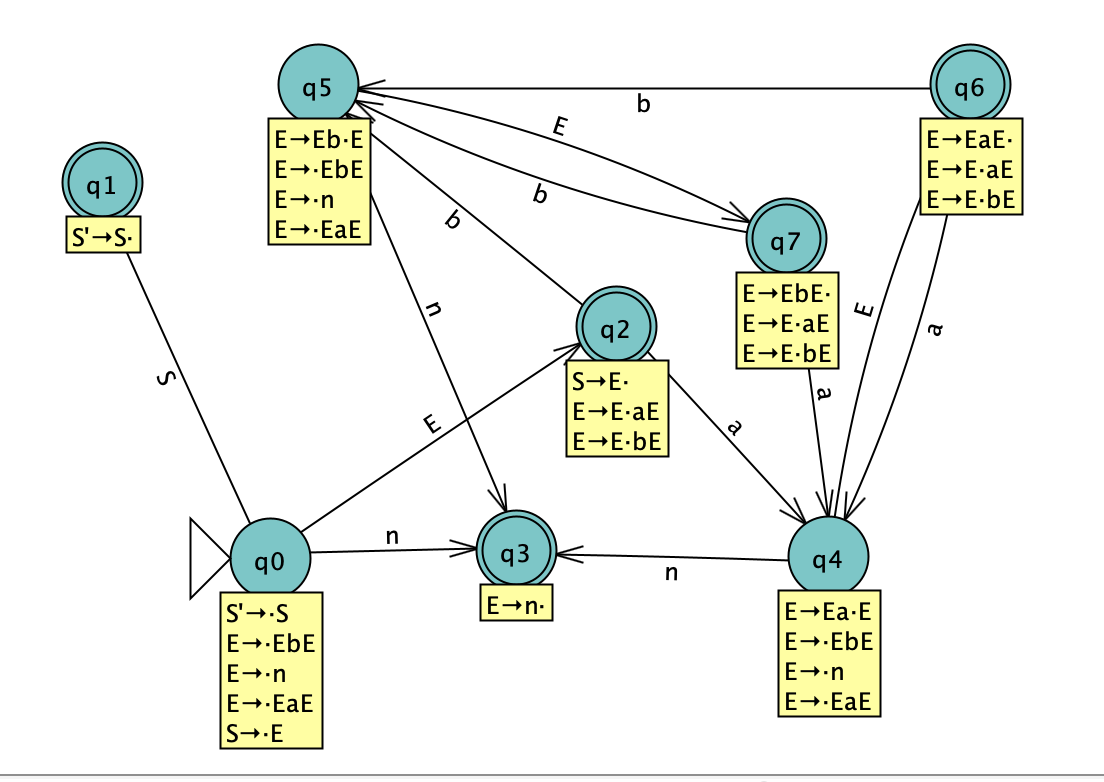
\includegraphics[width=0.8\textwidth]{./img/03AutomaSRL.png}
        \label{fig:03-automa}
    \end{figure}    
  \end{minipage}
  \hspace{0.2cm} 
  \begin{minipage}[t]{0.25\linewidth} 
    \subsection{First \& Follow}
    \begin{table}[H]
      \begin{tabular}{|c|c|c|}
      \hline
       & \textbf{First} & \textbf{Follow} \\
      \hline
      $S$ & $\{n\}$ & $\{\$\}$ \\
      \hline
      $E$ & $\{n\}$ & $\{a, b, \$\}$ \\
      \hline
      \end{tabular}
      \label{tab:03-first-follow}
    \end{table}
  \end{minipage}
\end{center}
\subsection{Tabella di parsing}
\begin{table}[H]
  \centering
  \begin{tabularx}{\textwidth}{|>{\centering\arraybackslash}X|>{\centering\arraybackslash}X|>{\centering\arraybackslash}X|>{\centering\arraybackslash}X|>{\centering\arraybackslash}X|>{\centering\arraybackslash}X|>{\centering\arraybackslash}X|}
  \hline
  \textbf{Stato} & \textbf{a} & \textbf{b} & \textbf{n} & \textbf{\$} & \textbf{E} & \textbf{S} \\
  \hline
  0 & & & S3 & & 2 & 1 \\
  \hline
  1 & & & & acc & & \\
  \hline
  2 & S4 & S5 & & R1 & & \\
  \hline
  3 & R2 & R2 & & R2 & & \\
  \hline
  4 & & & S3 & & 6 & \\
  \hline
  5 & & & S3 & & 7 & \\
  \hline
  6 & R3/\sout{S4} & R3/\sout{S5} & & R3 & & \\
  \hline
  7 & R4/\sout{S4} & R4/\sout{S5} & & R4 & & \\
  \hline
  \end{tabularx}
  \label{tab:03-parsing-table}
\end{table}
\subsection{Parsing}
Effettuiamo il parsing della parola $nbnan$:
\begin{table}[H]
  \begin{tabular}{lllll}
    \textbf{Parola} & \textbf{State Stack} & \textbf{Symbol Stack} & \textbf{Azioni} & \textbf{Regole Semantiche}\\
    \hline
    $nbnan$ & 0 &  \\
    $\underline n bnan$ & $03$ & $n$ & S3 & \\
    $\underline n bnan$ & $0\mathrel{\cancel 3}2$ & $\mathrel{\cancel  n} E$ & R2 G2 & $E.v = n.{lexval} = 4$\\
    $\underline {nb} nan$ & $025$ & $Eb$ & S5 & \\
    $\underline {nbn} an$ & $0253$ & $Ebn$ & S3 & \\
    $\underline {nbn} an$ & $025\mathrel{\cancel 3}7$ & $Eb\mathrel{\cancel  n}E$ & R2 G7 & $E.v = n.{lexval} = 3$\\
    $\underline {nbn} an$ & $0\mathrel{\cancel{257}}2$ & $\mathrel{\cancel{EbE}}E$ & R4 G2 & $E.v = E.v + E.v = 4 + 3 = 7$ \\
    $\underline {nbna} n$ & $024$ & $Ea$ & S4 & \\
    $\underline {nbnan} $ & $0243$ & $Ean$ & S3 & \\
    $\underline {nbnan} $ & $024\mathrel{\cancel 3} 6$ & $Ea\mathrel{\cancel  n} E$ & R2 G6 & $E.v = n.{lexval} = 3$ \\
    $\underline {nbnan} $ & $0\mathrel{\cancel{246}} 2$ & $\mathrel{\cancel{EaE}}E$ & R3 G6 & $E.v = E.v + E.v = 7 \cdot 3 = 21$ \\
    $\underline {nbnan} $ & $0\mathrel{\cancel 2}1$ & $\mathrel{\cancel E}S$ & R1 G1 & $S.v = E.v = 21$ \\
    $\underline {nbnan} $ & $01$ & $S$ & acc &  \\
  \end{tabular}
\label{tab:03-parsing-a}
\end{table}
\subsection{Risultato}
La valutazione della parola $4b3a3$ secondo la SDD $\mathcal S$ è 21.
\newpage
\section{Esercizio 4}
\subsection{Funzioni ed attributi}
\begin{itemize}
  \item \textit{node}: attributo sintetizzato che contiene informazioni sul tipo 
  (`+`, `*` o `id`), eventuali riferimenti alla tabella dei simboli e i 
  riferimenti ai figli del nodo, se presenti
  \item $newLeaf(\,label,\; value\,)$: funzione ausiliaria che va a creare 
  un nodo foglia, quindi per questa grammatica con label 'id' e value un 
  riferimento alla tabella dei simboli
  \item $newNode(\, label,\; child_1,\; child_2\,)$: funzione ausiliaria che 
  va a creare un nuovo nodo con label l'operatore (+ o *) e il riferimento
  ai nodi figli
\end{itemize}
\subsection{SDD}
\begin{center}
  \begin{minipage}[t]{0.29\linewidth}
    $E \rightarrow E_1 + E_2$ \\
    $E \rightarrow E_1 * E_2$ \\
    $E \rightarrow (E_1)$     \\
    $E \rightarrow id$     
  \end{minipage}
  \hspace{0.2cm}
  \begin{minipage}[t]{0.5\linewidth}
    \raggedright
    $\{E.node = newNode(\,'+',\; E_1.node,\; E_2.node\,);\}$ \\
    $\{E.node = newNode(\,'*',\; E_1.node,\; E_2.node\,);\}$ \\
    $\{E.node = E_1.node;\}$ \\
    $\{E.node = newLeaf(\,id,\; id.entry\,);\}$ \\
  \end{minipage}
  \hspace{0.2cm}
\end{center}
\section{Esercizio 5}
Riporto per comodità la SDT:
\begin{center}
  \begin{tabularx}{\linewidth}{m{0.25\linewidth} m{0.7\linewidth}}
  $S \rightarrow id = E$    & $\{gen(table.get(id) = E.addr);\}$ \\ [0.2cm]
  $S \rightarrow L = E$     & $\{gen(L.array.base[L.addr] = E.addr);\}$ \\ [0.2cm]
  $E \rightarrow E_1 * E_2$ & $\{E.addr = newTemp(); \quad gen(E.addr = E_1.addr \cdot E_2.addr);\}$ \\ [0.2cm]
  $E \rightarrow E_1 + E_2$ & $\{E.addr = newTemp(); \quad gen(E.addr = E_1.addr + E_2.addr);\}$ \\ [0.2cm]
  $E \rightarrow L$         & $\{E.addr = newTemp()\;\; \quad gen(E.addr = L.array.base[L.addr]);\}$ \\ [0.2cm]
  $E \rightarrow id$        & $\{gen(E.addr = table.get(id));\}$ \\ [0.4cm]
  $L \rightarrow id[E]$     & $\{L.array = table.get(id); \;\; L.type = arg2(table.getType(id)); \newline L.width = width(L.type);\;\; \newline L.addr = newTemp(); \quad \quad gen(L.addr = E.addr * L.width);\}$ \\ [1cm]
  $L \rightarrow L_1[E]$    & $\{L.array = L_1.array;\quad\quad L.type = arg2(L_1.type); \newline L.width = width(L.type);\newline t = newTemp(); \quad \quad \quad \quad gen(t = E.addr \cdot L.width);\newline L.addr = newTemp(); \quad \; \;\, gen(L.addr = t + L_1.addr);\}$ \\ [0.6cm]
  \end{tabularx}
\end{center}
A questo punto dobbiamo trovare l'albero di derivazione ed applicare le regole semantiche:
\begin{center}
  \begin{minipage}[t]{\linewidth}
    \begin{multicols}{3}
      \begin{figure}[H]
        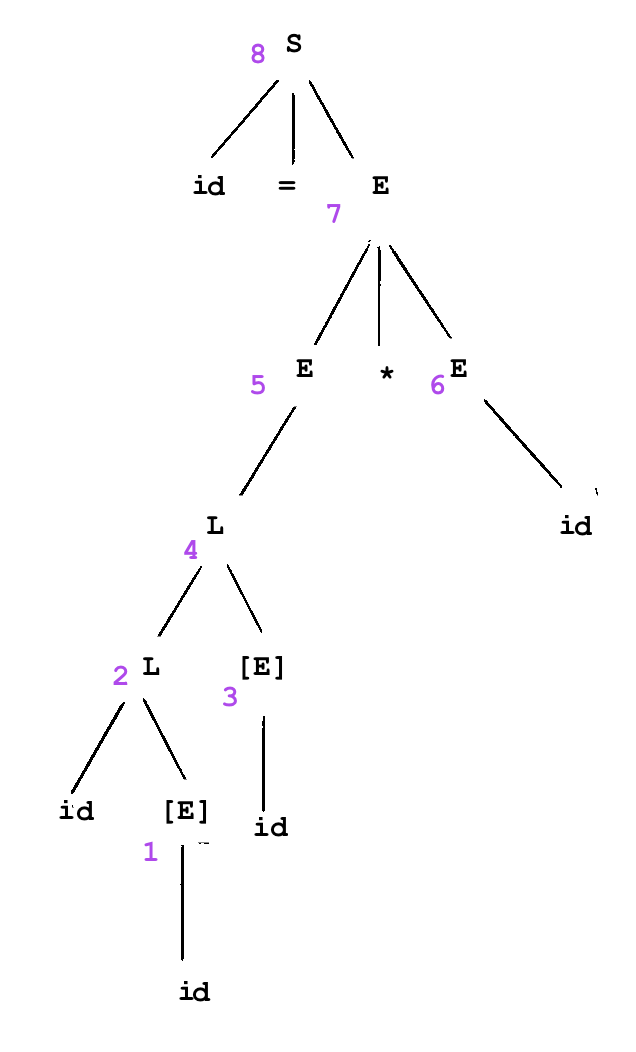
\includegraphics[height=6.2cm, width=5cm]{./img/05DerivationTree.png}
      \end{figure}
      \begin{enumerate}
        \item $E.addr = i$
        \item $L.array = a$ 
        \newline $L.type = array(3, integer)$
        \newline $L.width = 12$ {\color{teal} \quad \# [3 * 4]}
        \newline $L.addr = t_0$
        \newline {\color{red} $t_0 = i \cdot 12$}
        \item $E.addr = j$
        \item $L.array = a$
        \newline $L.type = int$
        \newline $L.width = 4$
        \newline $t_1 = newTemp()$
        \newline {\color{red} $t_1 = 4\cdot j$}
        \newline $L.addr = t_2$
        \newline {\color{red} $t_2 = t_0 + t_1$}
        \item $E.addr = t_3$
        \newline {\color{red} $t_3 = a[t_2]$} 
        \item $E.addr = c$
        \item $E.addr = t_4$
        \newline {\color{red} $t_4 = t_3 \cdot c$}
        \item {\color{red} $b = t_4$}
      \end{enumerate}
    \end{multicols}
  \end{minipage}
\end{center}

\section{Esercizio 6}
Per risolvere l'esercizio possiamo utilizzare la stessa SDT dell'esercizio precedente.
Per prima cosa costruiamo l'albero di derivazione per la stringa:
$$b =  c + a[i][j]$$
\begin{center}
  \begin{minipage}[t]{\linewidth}
    \begin{multicols}{2}
      \begin{figure}[H]
        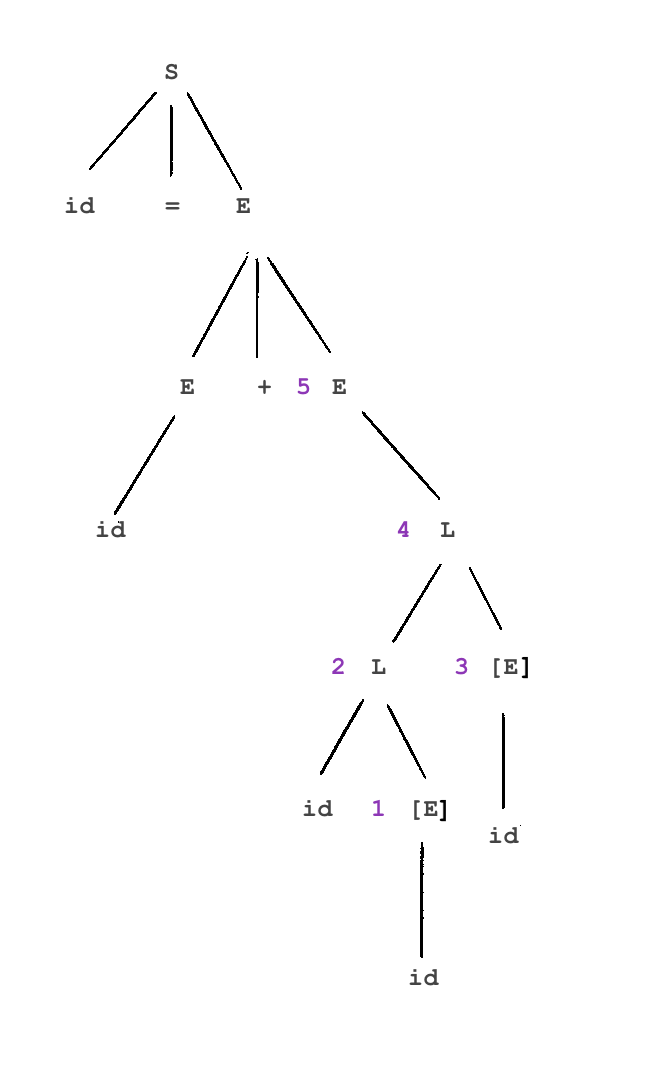
\includegraphics[height=10cm, width=7cm]{./img/06DerivationTree.png}
      \end{figure}
      Notiamo che non vi sono conflitti/ambiguità nel parsing di questa stringa, 
      quindi possiamo ottenere solo questo albero.
      \\La quinta riduzione è: $$E \rightarrow L$$
      \\Le sue regole semantiche sono: 
      \begin{itemize}
        \item $E.addr = newTemp();$
        \item $gen\big(E.addr = L.array.base[L.addr]\big);$
      \end{itemize}
      La seconda riduzione genererà un nuovo temporaneo $t_0$, 
      la quarta riduzione ne genererà altri due $t_1$ e $t_2$.
      \\Fatte queste assunzioni possiamo dire che il codice generato
      per questa riduzione sarà: $$t_3 = a[t_2]$$
      $$$$
    \end{multicols}
  \end{minipage}
\end{center}
\end{document}